\chapter{DESAIN DAN IMPLEMENTASI}
\label{chap:desainimplementasi}


\section{Struktur Rencana Kerja Pengembangan (WBS)}
\sloppy
Penelitian ini menggunakan pendekatan pengembangan berbasis \emph{Work Breakdown Structure} (WBS), yaitu metode sistematis untuk membagi keseluruhan proses pengembangan ke dalam unit-unit kerja yang lebih kecil dan terstruktur. WBS mencakup tahapan analisis kebutuhan, perancangan, implementasi, hingga evaluasi, yang disusun secara hierarkis untuk memudahkan perencanaan dan pelaksanaan sistem secara efisien. Diagram WBS yang digunakan dalam penelitian ini dapat dilihat pada Gambar \ref{fig:wbs}.

\begin{figure}[H]
  \centering
  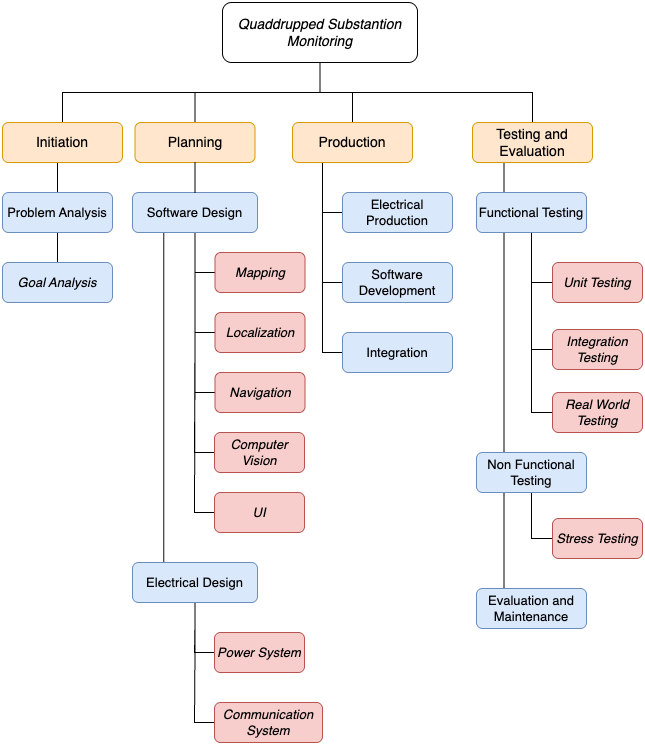
\includegraphics[width=0.8\textwidth]{gambar/bab3/wbs.png}
  \caption{\emph{Work Breakdown Structure} (WBS) Penelitian}
  \label{fig:wbs}
  \footnotesize{\textbf{Sumber:} Dokumentasi Pribadi}
\end{figure}

\section{Analisis Kebutuhan}
Analisis kebutuhan dilakukan melalui pengumpulan data dari studi literatur dan wawancara dengan pihak-pihak terkait. Berdasarkan hasil analisis. Adapun spesifikasi kebutuhan sistem yang harus dipenuhi dalam penelitian ini adalah sebagai berikut:

\begin{enumerate}
  \item Mengembangkan sistem \emph{computer vision} untuk mendeteksi dan mengidentifikasi komponen yang mengalami \emph{overheat} menggunakan kamera termal. Sistem ini juga harus mampu memperkirakan posisi dan jenis komponen yang terdeteksi mengalami \emph{overheat}.
  \item Merancang dan mengimplementasikan sistem navigasi otonom pada robot, sehingga robot dapat melakukan patroli secara mandiri di area gardu listrik, menghindari rintangan fisik, dan mengikuti jalur inspeksi yang telah ditentukan. Sistem navigasi ini harus beroperasi dengan stabil dan akurat di lingkungan yang memiliki gangguan elektromagnetik serta interferensi dari peralatan listrik.
  \item Merancang dan membangun \emph{control station} yang dapat memantau lokasi robot dan hasil deteksi \emph{overheat} secara \emph{real-time}.
\end{enumerate}


\section{Perancangan Sistem (\emph{Planning})}
Secara umum, perancangan sistem dibagi menjadi dua bagian utama, yaitu perancangan sistem elektrikal dan perangkat lunak. Perancangan sistem elektrikal mencakup desain sirkuit dan pemilihan komponen yang diperlukan untuk mendukung fungsi robot, sedangkan perancangan perangkat lunak mencakup pengembangan algoritma dan antarmuka pengguna yang akan digunakan dalam sistem.

\subsection{Desain Elektrikal}

Desain elektrikal robot mencakup perancangan sistem distribusi daya dan komunikasi yang bertujuan untuk mengintegrasikan komponen-komponen tambahan ke dalam sistem robot yang telah ada. Komponen tambahan ini dirancang untuk mendukung kapabilitas operasi otonom robot secara menyeluruh. Rancangan lengkap dari sistem dapat dilihat pada Gambar~\ref{fig:electrical}.

\begin{figure}[H]
  \centering
  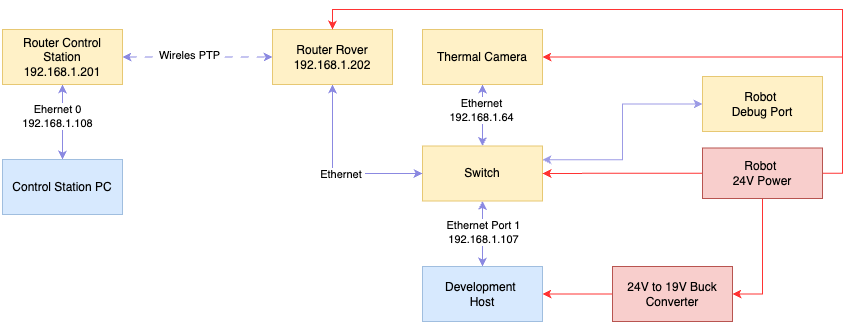
\includegraphics[width=1\textwidth]{gambar/bab3/electrical.png}
  \caption{Desain Elektrikal Robot}
  \label{fig:electrical}
  \footnotesize{\textbf{Sumber:} Dokumentasi Pribadi}
\end{figure}

Pada Gambar~\ref{fig:electrical}, terlihat bahwa robot dilengkapi dengan sejumlah komponen tambahan, antara lain kamera termal, modul komunikasi nirkabel, \emph{switch} jaringan, dan \emph{development host}. Kamera termal yang digunakan membutuhkan suplai daya sebesar 24~VDC, sedangkan \emph{development host} menggunakan tegangan 12~VDC. Oleh karena itu, sistem dilengkapi dengan konverter penurun tegangan dari 24~VDC ke 12~VDC untuk memenuhi kebutuhan perangkat tersebut. Seluruh komponen lainnya disuplai langsung dari sistem kelistrikan utama 24~VDC robot. Dari sisi komunikasi internal, semua perangkat terhubung melalui \emph{switch} jaringan yang kemudian terintegrasi ke dalam sistem robot melalui \emph{debug port}, sehingga membentuk satu jaringan lokal tertutup yang mendukung komunikasi data antar perangkat secara stabil.

Untuk komunikasi eksternal dengan \emph{control station}, digunakan skema komunikasi \emph{Point-to-Point} (PTP) berbasis nirkabel pada frekuensi 5{,}8~GHz. Dalam konfigurasi ini, unit pemancar yang terpasang pada \emph{control station} dikonfigurasi sebagai \emph{access point} (AP), sedangkan unit pada robot berfungsi sebagai \emph{station}. Skema ini memungkinkan pertukaran data dua arah berkecepatan tinggi dengan latensi rendah, yang sangat penting untuk transmisi data sensor, video termal, serta komando kendali secara \emph{real-time}.



\subsection{Desain Perangkat Lunak Robot}
Desain perangkat lunak pada robot dilakukan dengan mempertimbangkan arsitektur perangkat lunak yang bersifat modular dan terintegrasi. Pendekatan ini bertujuan untuk mempermudah proses pengembangan, pemeliharaan, serta pengujian sistem secara menyeluruh. Dalam penelitian ini, perangkat lunak dibagi menjadi beberapa \textit{package} ROS yang masing-masing memiliki fungsi spesifik dan saling terhubung.

Terdapat empat \textit{package} utama yang dikembangkan, yaitu \textit{IO package}, \textit{Localization and Mapping package}, \textit{Autonomy package}, dan \textit{Perception package}. Struktur umum dari arsitektur perangkat lunak ini dapat dilihat pada Gambar~\ref{fig:software-arch}.

\begin{figure}[H]
  \centering
  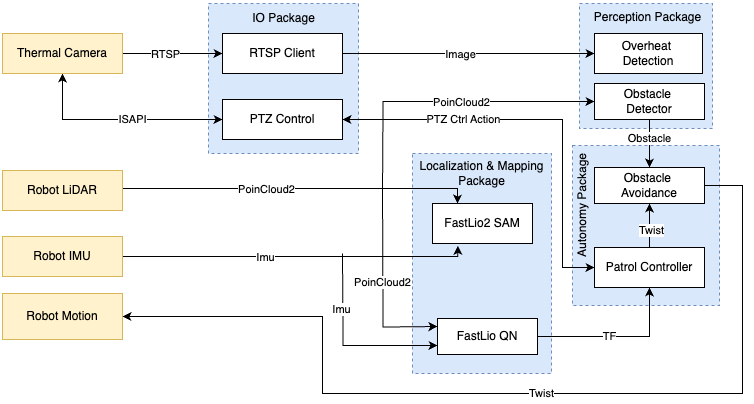
\includegraphics[width=0.9\textwidth]{gambar/bab3/sftware-arch.png}
  \caption{Arsitektur Perangkat Lunak Robot}
  \label{fig:software-arch}
  \footnotesize{\textbf{Sumber:} Dokumentasi Pribadi}
\end{figure}

Setiap \textit{package} menjalankan fungsi tertentu dan saling berkomunikasi melalui mekanisme \textit{topic}, \textit{service}, atau \textit{action} sesuai dengan kebutuhan sistem.

\subsubsection{3.3.2.1 \emph{IO Package}}
\textit{IO package} bertanggung jawab untuk mengelola seluruh input dan output dari perangkat keras robot, yang dalam hal ini adalah kamera thermal. \textit{IO package} terdiri dari dua program utama, yaitu \textit{RTSP client} dan \textit{PTZ controller}.  \textit{RTSP client} berfungsi untuk menghubungkan kamera thermal dengan sistem robot dan mengubah aliran data menjadi \textit{rostopic} berupa \textit{compressed image}. Sementara itu, \textit{PTZ controller} digunakan untuk mengatur pergerakan \textit{pan-tilt-zoom} (PTZ) serta menerima status posisi PTZ saat ini menggunakan protokol ISAPI. Informasi ini kemudian digunakan untuk mengontrol pergerakan PTZ secara dinamis, yang dipadukan dengan \textit{PID controller} untuk memperoleh kecepatan rotasi dan sudut target yang akurat.

\subsubsection{3.3.2.2 \emph{Localization and Mapping Package}}
\emph{Localization and Mapping package} bertanggung jawab untuk menentukan estimasi posisi robot secara \emph{real-time} dalam peta serta memperbarui peta berdasarkan data sensor yang diterima. Dalam sistem ini, proses pelokalan dan pemetaan dilakukan secara terpisah namun saling terintegrasi, sesuai dengan pendekatan \emph{frontend-backend} pada sistem \emph{SLAM} modern. Sebagaimana dijelaskan dalam tinjauan pustaka (lihat Subbab 2.2.5.4 dan 2.2.5.5), proses pemetaan awal dilakukan menggunakan \emph{Fast-LIO-SAM}, yaitu kombinasi dari \emph{LiDAR-Inertial Odometry (LIO)} dan \emph{backend} optimisasi graf berbasis \emph{Smoothing and Mapping (SAM)}. Hasil dari proses ini adalah peta lingkungan tiga dimensi yang disimpan dalam format file \texttt{.bag}. Peta ini kemudian digunakan sebagai referensi statis untuk proses lokalisasi.

Pada proses lokalisasi, digunakan \emph{Fast-LIO Localization QN}, sebuah sistem lokalisasi berbasis peta yang menggabungkan estimasi \emph{odometry} dari \emph{Fast-LIO2} dengan algoritma pencocokan peta \emph{Quatro} dan \emph{NanoGICP}. Modul \emph{Quatro} digunakan untuk estimasi kasar posisi awal, sedangkan \emph{NanoGICP} melakukan penyempurnaan transformasi posisi secara lokal dengan presisi tinggi dan efisiensi komputasi yang optimal.Koordinat posisi robot hasil proses lokalisasi akan dipublikasikan dalam sistem \emph{ROS} melalui transformasi koordinat (\emph{tf}) menggunakan modul \emph{tf broadcaster}. Dengan pendekatan ini, sistem mampu melakukan navigasi berbasis peta secara efisien tanpa perlu membangun ulang peta di setiap sesi operasi, serta mendukung inisialisasi cepat dalam lingkungan yang telah dipetakan sebelumnya.


\subsubsection{3.3.2.4 \emph{Perception Package}}

\emph{Perception package} bertanggung jawab untuk melakukan estimasi posisi komponen yang mengalami panas berlebih (\emph{overheat}) pada gardu listrik. Proses ini terdiri dari beberapa tahapan yang saling terintegrasi. Tahapan pertama dimulai dari pemrosesan citra termal yang diperoleh dari kamera termal. Kamera ini secara otomatis menyediakan informasi suhu tertinggi dan terendah dari setiap frame citra yang ditangkap, dan data tersebut dapat diakses melalui protokol \emph{ISAPI}. Suhu tertinggi pada citra digunakan sebagai indikator awal keberadaan komponen yang berpotensi mengalami \emph{overheat}. Jika suhu tertinggi ini melampaui ambang batas tertentu yang telah ditetapkan, maka sistem akan melanjutkan ke tahapan berikutnya. Pada tahap selanjutnya, sistem melakukan deteksi objek menggunakan algoritma \emph{YOLOv8} untuk mengidentifikasi keberadaan komponen pada citra termal. Jika algoritma ini berhasil mendeteksi kelas komponen yang mengalami overheat pada suhu tertinggi yang terdeteki pada \emph{frame} maka sistem akan mengonfirmasi status \emph{overheat} dari komponen tersebut dengan membaca suhu aktual dari objek tersebut. Apabila suhu tersebut melebihi ambang batas yang ditentukan, sistem akan melakukan estimasi posisi spasial dari komponen tersebut. Estimasi posisi diperoleh dengan menggabungkan informasi sudut pandang kamera (\emph{angle of view}) dan orientasi vertikal kamera (\emph{tilt}) yang disejajarkan dengan bidang pemindaian \emph{LiDAR}. Jarak hasil pemindaian dari \emph{LiDAR} kemudian digunakan sebagai acuan untuk menghitung posisi spasial objek dalam koordinat lingkungan nyata.

Di sisi lain, sistem \emph{obstacle detector} pada robot menghasilkan sebanyak 30 garis deteksi yang tersebar dalam sudut 180 derajat dari sisi kiri ke arah depan robot seperti pada gambae 
\begin{figure}[H]
  \centering
  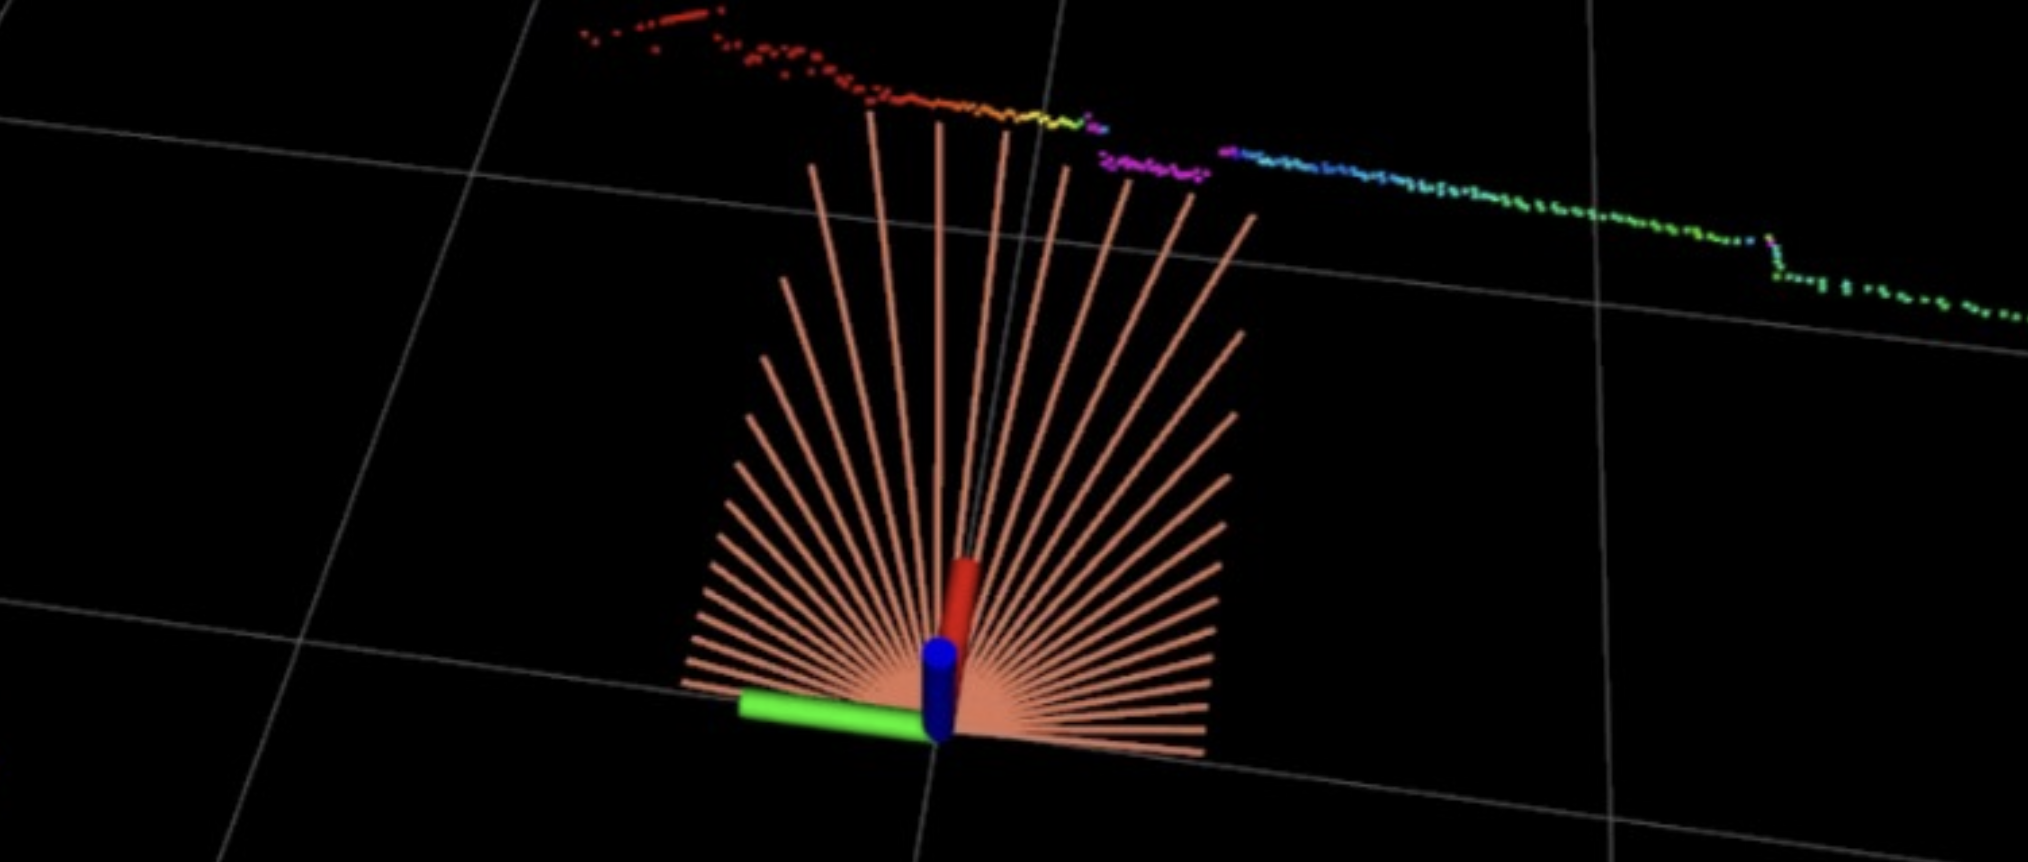
\includegraphics[width=0.9\textwidth]{gambar/bab3/obstacle_avoidance.png}
  \caption{Visualisasi Garis Deteksi Rintangan pada RViz}
  \label{fig:obstacle-avoidance}
  \footnotesize{\textbf{Sumber:} Dokumentasi Pribadi}
\end{figure}




Masing-masing garis memiliki bobot atau nilai \emph{multiplier} yang berbeda, yang digunakan untuk menilai tingkat risiko dan menentukan keputusan gerakan. Ketika terdeteksi objek di salah satu arah, sistem akan mengevaluasi apakah robot harus melanjutkan pergerakan maju atau melakukan manuver penghindaran, tergantung pada distribusi dan kedekatan objek di sekitar jalur. Informasi hasil  deteksi rintangan, akan diteruskan ke \emph{autonomy package} sebagai masukan untuk pengambilan keputusan navigasi secara otonom. Dengan pendekatan ini, sistem mampu melakukan deteksi serta identifikasi objek secara efisien, dan memberikan kontribusi penting dalam memastikan keselamatan serta efektivitas pergerakan robot di lingkungan nyata.

\subsubsection{3.2.2.3 \emph{Autonomy Package}}


Dalam sistem \emph{autonomy}, yang pada dasarnya merupakan proses navigasi jalur, lintasan robot diperoleh dari hasil perekaman \emph{path} yang dilakukan pada saat proses pemetaan. Jalur ini kemudian disimpan dalam format \texttt{.json}, baik secara lokal maupun melalui pada database \emph{control station}. Integrasi antara pengendalian lintasan dan penghindaran rintangan menjadi aspek yang krusial dalam sistem ini. Salah satu strategi yang umum digunakan adalah mengimplementasikan algoritma \emph{PID} atau \emph{Pure Pursuit} sebagai pengendali utama lintasan, sementara modul penghindaran rintangan berbasis \emph{Braitenberg} diaktifkan secara kondisional ketika objek terdeteksi dalam jarak tertentu. Pendekatan ini memungkinkan robot untuk tetap mengikuti jalur yang telah direkam, namun tetap mampu bereaksi secara dinamis terhadap rintangan tanpa harus melakukan perencanaan ulang lintasan secara menyeluruh. Integrasi semacam ini dapat direalisasikan melalui skema \emph{behavior-based arbitration} atau \emph{subsumption architecture}, di mana modul penghindaran rintangan memiliki prioritas lebih tinggi ketika kondisi kritis terdeteksi. Setelah lingkungan kembali aman, kontrol akan dialihkan kembali ke pengendali lintasan utama. Dengan pendekatan ini, sistem navigasi menjadi lebih adaptif, aman, dan efisien, terutama dalam menghadapi lingkungan nyata yang dinamis.


\subsubsection{3.3.2.4 \emph{Computer Vision}}

\emph{Computer vision} merupakan salah satu komponen dari \emph{perception package} yang bertanggung jawab untuk mendeteksi jenis komponen dan mengestimasi suhunya berdasarkan citra termal. Proses ini dilakukan dengan menggabungkan algoritma deteksi objek berbasis \emph{YOLOv8} dan analisis suhu menggunakan segmentasi dalam ruang warna \emph{grayscale}. Sistem \emph{computer vision} dikembangkan untuk mendeteksi, mengklasifikasi, dan memperkirakan suhu dari komponen yang teridentifikasi pada citra termal, dengan tujuan meningkatkan efisiensi serta akurasi dalam mendeteksi kondisi \emph{overheat} pada komponen gardu listrik.

Model \emph{YOLOv8} dipilih karena kemampuannya dalam melakukan deteksi objek secara akurat dan cepat. Setelah objek terdeteksi, suhu pada setiap komponen dievaluasi untuk menentukan apakah terjadi kondisi \emph{overheat}. Deteksi suhu dilakukan berdasarkan analisis warna dalam citra termal pada area \emph{bounding box} hasil deteksi objek. Proses ini sangat penting karena masing-masing komponen memiliki ambang batas suhu kritis yang berbeda-beda. Oleh karena itu, proses identifikasi objek dilakukan terlebih dahulu untuk memastikan interpretasi suhu yang relevan dan akurat. Proses \emph{computer vision} ini terdiri dari beberapa tahapan, yaitu:

\subsubsection*{A. Pembuatan Dataset}
Dataset citra termal dari komponen gardu listrik dikumpulkan dan dianotasi secara manual menggunakan platform \emph{Roboflow}. Setiap citra diberi label yang merepresentasikan jenis komponen secara akurat, yang kemudian digunakan sebagai data latih untuk model deteksi objek.

\subsubsection*{B. Pelatihan Model \emph{YOLOv8}}
Model \emph{YOLOv8} dilatih menggunakan dataset citra termal yang telah melalui proses anotasi dan \emph{preprocessing}. Selama proses pelatihan, dilakukan penyesuaian \emph{hyperparameter} seperti \emph{learning rate}, ukuran batch, dan jumlah epoch untuk mencapai hasil yang optimal. Selain itu, teknik augmentasi data seperti rotasi, flipping horizontal, dan perubahan intensitas cahaya juga diterapkan guna meningkatkan kemampuan generalisasi model terhadap variasi kondisi lapangan. Setelah proses pelatihan selesai, model divalidasi menggunakan dataset uji yang terpisah dari data pelatihan untuk menghindari bias dan memastikan bahwa model memiliki kinerja yang stabil dan dapat diandalkan dalam skenario dunia nyata.


\subsubsection*{C. Konversi ke \emph{OpenVINO}}
Setelah model \emph{YOLOv8} dilatih dan tervalidasi, tahap berikutnya adalah melakukan konversi ke format \emph{OpenVINO}. Tujuan konversi ini adalah untuk mengoptimalkan inferensi model agar dapat dijalankan secara efisien pada perangkat keras dengan sumber daya terbatas, seperti komputer embedded atau sistem robotik industri.

\subsubsection*{D. Inferensi \emph{YOLOv8}}
Inferensi dilakukan dengan menggunakan model \emph{YOLOv8} yang telah terlatih dan dikonversi ke format \emph{OpenVINO}. Proses inferensi ini bertujuan untuk mendeteksi objek pada citra termal yang diambil oleh kamera. Hasil dari inferensi ini adalah koordinat \emph{bounding box} yang mengelilingi objek yang terdeteksi, serta kelas objek tersebut. Dengan informasi ini, sistem dapat mengidentifikasi jenis komponen yang terdeketsi pada frame citra termal. Proses inferensi dilakukan secara \emph{real-time}. Selain itu, sistem juga melakukan pengolahan citra tambahan untuk meningkatkan akurasi deteksi, seperti penyesuaian kontras dan pencahayaan pada citra termal sebelum dilakukan inferensi.
\subsubsection*{E. Deteksi Kelas dan Suhu Komponen}
Setelah komponen berhasil terdeteksi oleh \emph{YOLOv8}, tahap selanjutnya adalah menganalisis suhu dari setiap objek pada area \emph{bounding box}. Analisis dilakukan dengan mengubah citra termal ke dalam format \emph{grayscale}. Suhu tinggi biasanya direpresentasikan dengan warna cerah yang akan memikiki intensitas tinggi pada citra \emph{grayscale}. Dengan menggunakan metode segmentasi, sistem dapat mengidentifikasi area dengan suhu tinggi dan menghitung nilai rata-rata suhu pada area tersebut. Proses ini dilakukan dengan memanfaatkan informasi suhu tertinggi yang diperoleh dari kamera termal, yang kemudian digunakan sebagai acuan untuk menentukan ambang batas suhu pada objek yang terdeteksi.


\subsection{Desain \textit{Control Station}}

\emph{Control station} merupakan pusat kendali dan pemantauan dari sistem robot. Dalam penelitian ini, \emph{control station} dirancang untuk memantau lokasi robot dan hasil deteksi \emph{overheat} secara \emph{real-time}. Sistem ini dikembangkan menggunakan framework \emph{Next.js} pada sisi \emph{frontend}, dengan tampilan antarmuka yang dirancang menggunakan \emph{Tailwind CSS} dan pustaka komponen \emph{shadcn/ui}. Kombinasi ini menghasilkan desain antarmuka yang modern, responsif, dan mudah digunakan oleh operator di lapangan. Pada sisi \emph{backend}, sistem menggunakan \emph{Express.js} sebagai penyedia \emph{REST API} yang mengelola komunikasi antara antarmuka pengguna dan perangkat robot. Seluruh data operasional disimpan dalam basis data \emph{PostgreSQL}, yang mencakup informasi pengguna, lintasan patroli (\emph{path}), posisi robot, serta titik koordinat deteksi komponen yang mengalami \emph{overheat}. Pertukaran data antara robot dan \emph{control station} dilakukan secara efisien melalui protokol \emph{WebSocket} dan \emph{HTTP} untuk memastikan komunikasi \emph{real-time} yang stabil.
\begin{figure}[H]
  \centering
  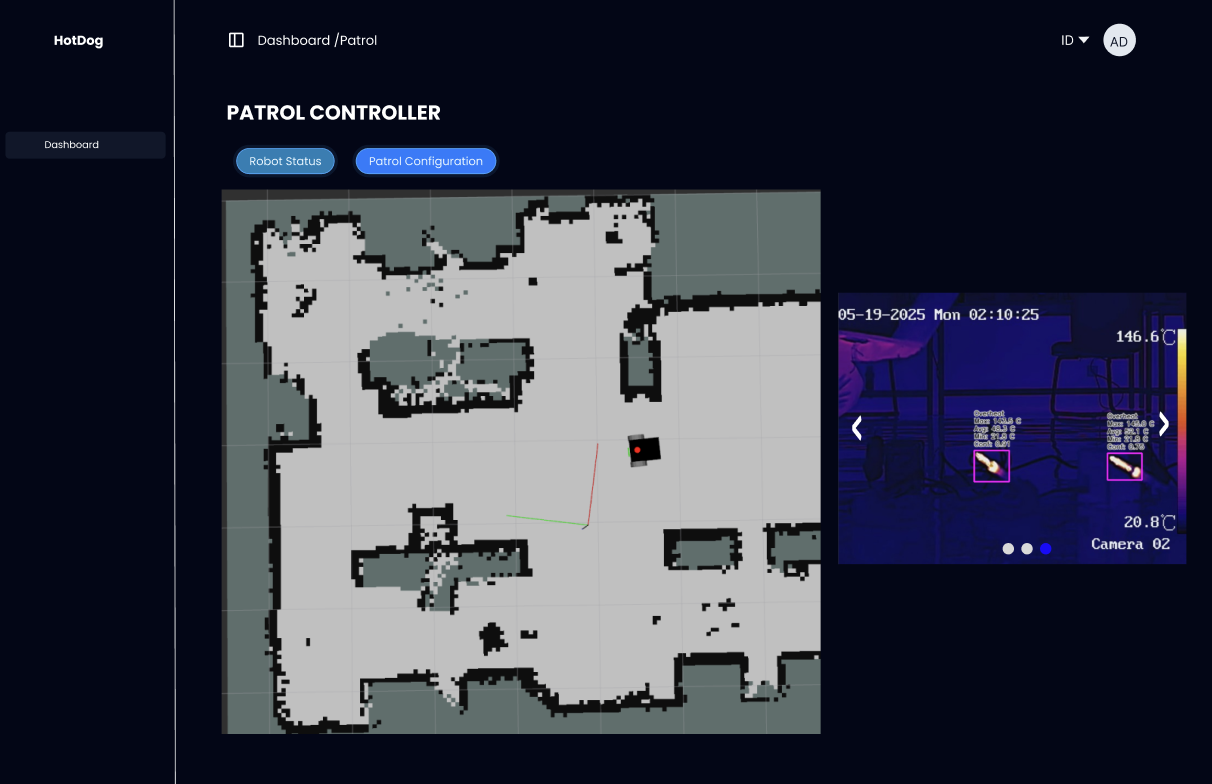
\includegraphics[width=0.6\textwidth]{gambar/bab3/control-station.png}
  \caption{Desain Antarmuka Pengguna \emph{Control Station}}
  \label{fig:control-station}
  \footnotesize{\textbf{Sumber:} Dokumentasi Pribadi}
\end{figure}

Antarmuka pengguna \emph{control station} mencakup dua komponen utama yang terintegrasi. Komponen pertama adalah status robot, yang menampilkan posisi terkini robot dalam peta bentuk \emph{grid map}, lengkap dengan titik lokasi komponen yang terdeteksi mengalami \emph{overheat}. Setiap titik ditandai komponen akan memikiki image dan keterangan suhu serta berdasarkan suhu dan waktu deteksi. Komponen kedua adalah konfigurasi patroli, yang menampilkan daftar lintasan yang tersedia dan informasi terkait rute patroli yang sedang dijalankan oleh robot. Jalur yang dipilih akan divisualisasikan secara dinamis, memungkinkan operator untuk memantau progres pergerakan robot dan melakukan intervensi bila diperlukan. 